\chapter{SkylineLab}
\label{ch:skylinelab}

\begin{preamble}
This assignment is designed to give you more practice with divide-and-conquer
algorithms as well as provide an introduction to using the sequence function
\sml{scan}. You will analyze and solve the \emph{skyline problem}, which is a
geometric problem in 2 dimensions. This lab is conceptually difficult, so be
sure to get started early!
\end{preamble}

\section{Files}

\begin{gram}
\begin{filesInstructions}{skylinelab}
  \filestar{MkSkyline.sml}
  \file{Sandbox.sml}
  \file{Tests.sml}
\end{filesInstructions}
\end{gram}

\section{Submission}

\begin{gram}
\makeSubmissionInstructions{SkylineLab}
\end{gram}

\section{The Skyline Problem}

\begin{gram}
\begin{center}
  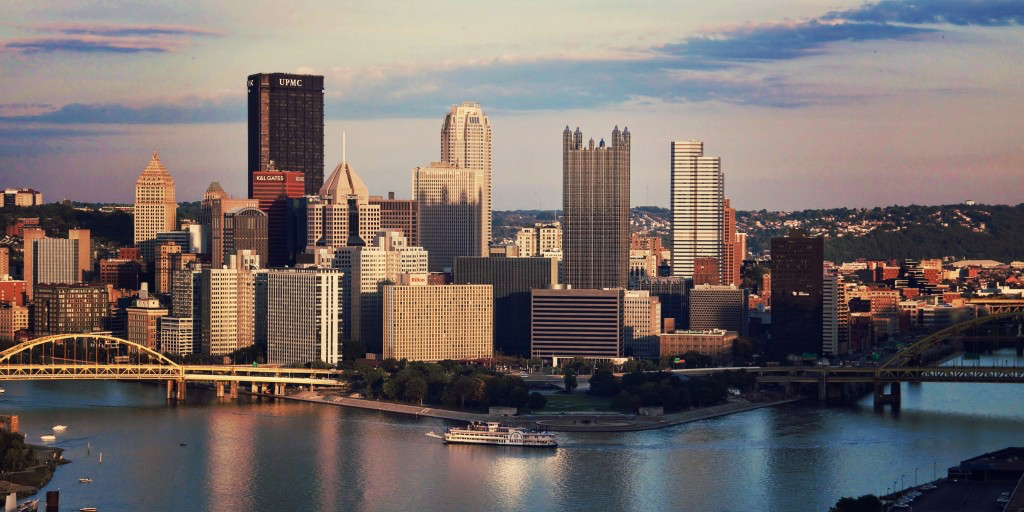
\includegraphics[width=5in]{./skyline/media/pittsburgh.png}
\end{center}

Feast your eyes upon downtown Pittsburgh. From our perspective, most
of the buildings are roughly rectangular (the exceptions being those like PPG
Place), so let's assume from now on that all buildings are rectangles. We'll
also assume that the ground is perfectly flat so that all the rectangles rest
on the same line. The \emph{skyline} of these rectangles is their
silhouette.


\begin{center}
  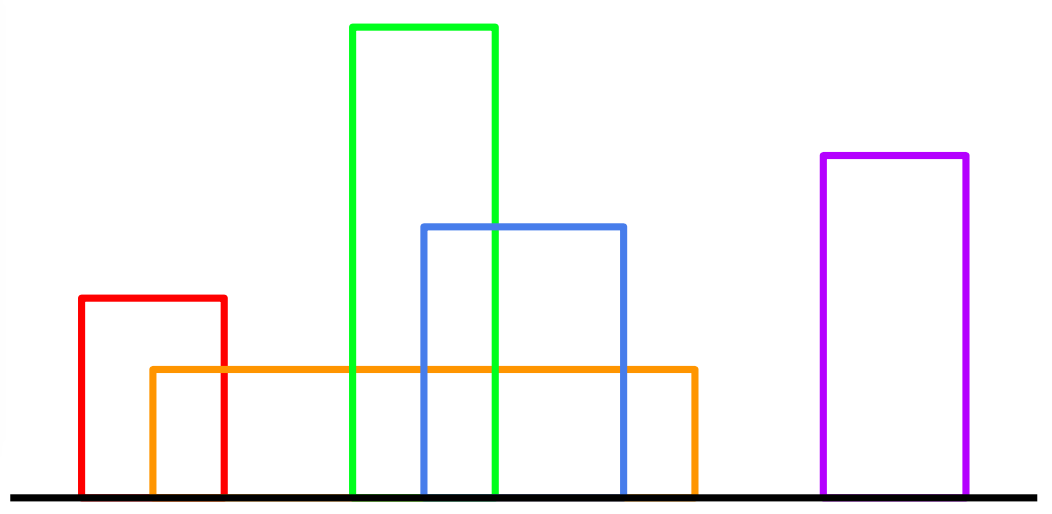
\includegraphics[width=5in]{./skyline/media/buildings.png}

  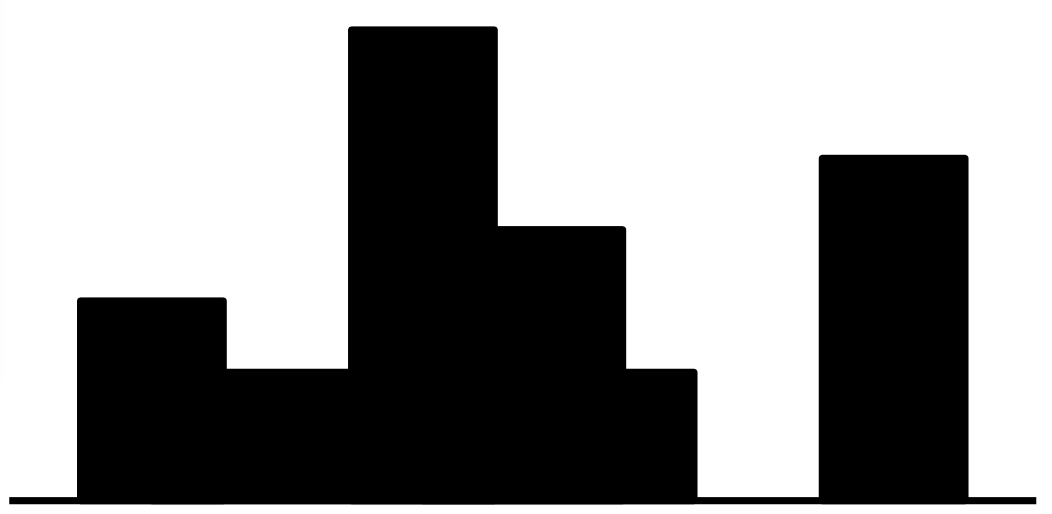
\includegraphics[width=5in]{./skyline/media/silhouette.png}

\end{center}
\end{gram}

\begin{gram}[Buildings]
Under the assumptions given, each building can be represented by a triple
$(\ell,h,r)$ which describes a rectangle with corners $(\ell, 0)$, $(\ell, h)$,
$(r, h)$, and $(r, 0)$. We will assume $\ell < r$ so that $\ell$ and $r$ are
the left and right sides of the building, and $h$ is the height of the building.
\end{gram}

\begin{definition}
The skyline of a set of buildings $B$ is
\[ \left\{ (x, H(x)) : x \in X\ \Big|\
   x = \min X \;\lor\; H(x) \neq H(\text{prev}(x)) \right\} \]
where $X$ is the set of all $x$-coordinates in $B$, $H(x)$ is the max height
at $x$, and $\text{prev}(x)$ is the nearest $x'$ to the left of $x$, given by
\begin{align*}
  X &= \bigcup_{(\ell,h,r) \in B} \{\ell, r\} \\
  H(x) &= \max \big\{ h : (\ell, h, r) \in B\ \big|\ \ell \leq x < r \big\} \\
  \text{prev}(x) &= \max \big\{ x' \in X\ \big|\ x' < x \big\}
\end{align*}

In other words, the $x$-coordinates in the skyline are exactly those which
appear in $B$, and the $y$-coordinate for any particular $x$ is the height $h$
of the tallest building $(\ell, h, r)$ for which $\ell \leq x < r$. We do not
include \textbf{redundant} points: points whose height is unchanged from the
nearest point to the left.
\end{definition}

\begin{example}
Buildings:
\begin{tabular}[t]{ccc}
  $\ell$ & $h$ & $r$ \\\hline
  2 & 3 & 4 \\
  3 & 2 & 11 \\
  6 & 7 & 8 \\
  7 & 4 & 10 \\
  13 & 5 & 15 \\
\end{tabular}

Skyline:
\begin{tabular}[t]{cc}
  $x$ & $y$ \\\hline
  2 & 3 \\
% 3 & 3 \\ % duplicate
  4 & 2 \\
  6 & 7 \\
% 7 & 7 \\ % duplicate
  8 & 4 \\
  10 & 2 \\
  11 & 0 \\
  13 & 5 \\
  15 & 0 \\
\end{tabular}

In the diagrams below, skyline points are marked with

\includegraphics[width=0.2in]{./skyline/media/circ.png}. Redundant points are
marked in the first diagram with

\includegraphics[width=0.2in]{./skyline/media/x.png}.

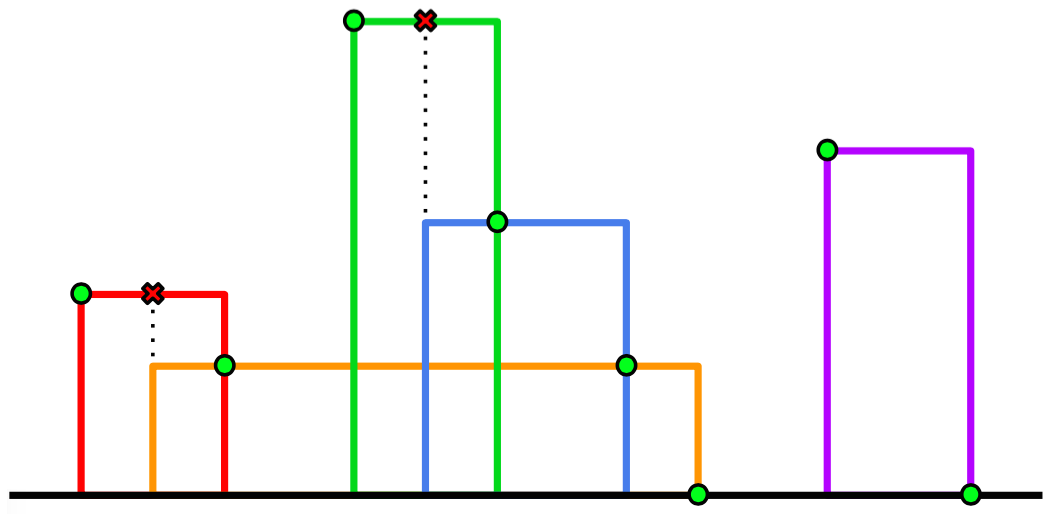
\includegraphics[width=5in]{./skyline/media/skyline.png}

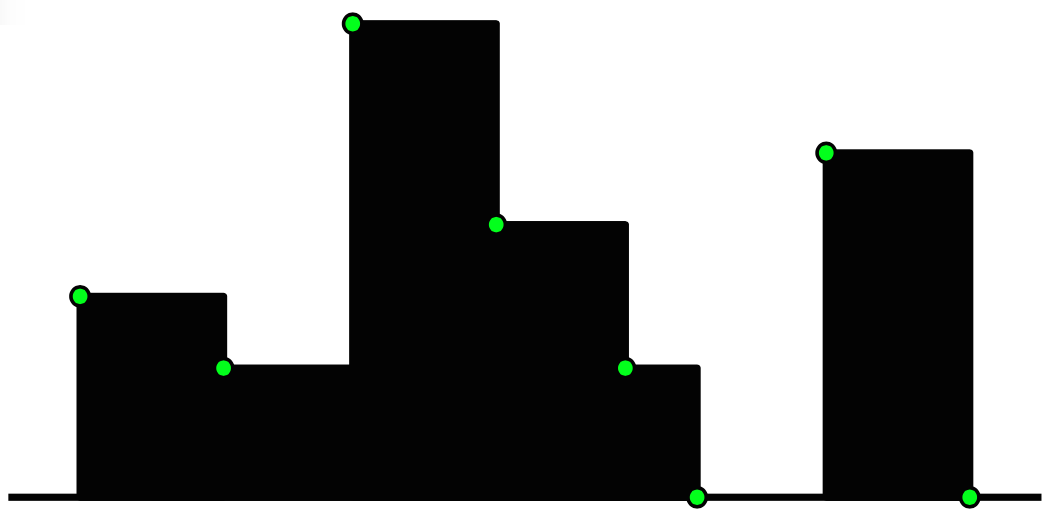
\includegraphics[width=5in]{./skyline/media/silhouette-points.png}
\end{example}


\subsection{Implementation}

We define \sml{type skyline = (int * int) Seq.t}. We maintain the convention
that all skylines are \textbf{sorted by $x$-coordinate}, and \textbf{do not
contain redundant points}. Throughout, we assume that all $x$-coordinates are
unique and non-negative, and that all heights are strictly positive.

Given a sequence of buildings $B$ in no particular order, your goal is to write
a divide-and-conquer algorithm for the skyline problem of the following form:
\begin{verbatim}
fun skyline B =
  case Seq.splitMid B of
    Seq.EMPTY => Seq.empty ()
  | Seq.ONE x => singleton x
  | Seq.PAIR (L, R) =>
      combine (Primitives.par (fn () => skyline L,
                               fn () => skyline R))
\end{verbatim}
\sml{singleton} has been implemented for you in \sml{MkSkyline.sml} and has
constant work and span. All you have to do is implement \sml{combine}.

\begin{note}
You may assume all $x$-coordinates in $B$ are unique.
\end{note}

\begin{remark}
The behavior of this code is identical to the following, which uses
\sml{reduce} to ``automate'' the divide-and-conquer process.
\begin{verbatim}
fun skyline B =
  Seq.reduce combine (Seq.empty ()) (Seq.map singleton B)
\end{verbatim}
\end{remark}

\begin{task}[1]
\label{task:skylinelab:1}
(60 points)
In \texttt{MkSkyline.sml}, implement the following function.
\begin{verbatim}
val combine : skyline * skyline -> skyline
\end{verbatim}
\sml{combine (S1, S2)} should evaluate to the skyline of all buildings
from both $S_1$ and $S_2$. Your implementation must have $\bigO {|S_1| + |S_2|}$ work
and $\bigO {\log|S_1| + \log|S_2|}$ span.
\end{task}

\begin{hint}
You will probably find the functions \sml{merge},
\sml{scan}/\sml{scanIncl}, and \sml{filter}/\sml{filterIdx}
useful. In particular, take a close look at \sml{scan}.
For constant-work functions $f$, \sml{scan f b s} has $O(|s|)$ work and
$O(\log|s|)$ span. The cost bounds of \sml{scanIncl} are identical.
\end{hint}

\begin{important}
In \sml{scan f b s}, the function $f$ must be \emph{associative}, meaning that
for all inputs $a,b,c$,
\[ f(f(a,b),c) = f(a,f(b,c)) \]
\end{important}

\begin{note}
As usual, assume $\sml{Seq} = \sml{ArraySequence}$ for cost analysis.
\end{note}

\begin{note}
Don't forget about removing redundant points!
\end{note}

\subsection{Testing}

It is very important that you thoroughly test your code before you
submit. After the deadline, we will grade your code with a private set of test
cases.

We provide two ways to test your code with SML/NJ.
\begin{enumerate}
  \item
  In \texttt{Sandbox.sml}, write whatever testing code you'd like. You can then
  access the sandbox at the REPL:
\begin{verbatim}
- CM.make "sandbox.cm";
...
- open Sandbox;
\end{verbatim}
%
  \item
  In \texttt{Tests.sml}, add test cases according to the instructions given.
  Then run the autograder:
\begin{verbatim}
- CM.make "autograder.cm";
...
- Autograder.run ();
\end{verbatim}
\end{enumerate}


\section{Performance Evaluation}

\begin{note}
All tasks in this section should be included in your \texttt{written.pdf}
submitted to Gradescope.
\end{note}


How efficient is your parallel code? To answer this question, we might begin by
splitting it into two distinct issues:
%
\begin{enumerate}
\item How parallel is your code? That is, how much faster does it get as we use more processors?
\item How much extra work does your code do, in order to be parallel?
\end{enumerate}


\subsection{Introduction and Definitions}
\label{subsub:defns}

We can tackle these questions by measuring speedup and overhead. In particular,
for a fixed input, let $T^*$ be the amount of time it takes to solve that
input using a fast sequential program, and let $T_P$ be the amount of time it
takes your parallel program on $P$ processors (and similarly $T_1$ is your program's
runtime on 1 processor). We can then compute:
%
\begin{enumerate}
\item The self-speedup on $P$ processors, $T_1 / T_P$.
\item The overhead, $T_1 / T^*$.
\end{enumerate}

\begin{task}[2]
(5 points)
Ideally, what is a lower bound on $T_P$? Consequently, what is an upper bound on
the self-speedup on $P$ processors? Give your answers in terms of $P$ and $T_1$.
\end{task}

\begin{task}[3]
(5 points)
Is $T_1$ an upper bound on $T^*$? Briefly justify your answer.
\end{task}

\subsection{Experiments}

\begin{flex}

You will now experimentally measure $T^*$, $T_1$, and $T_P$. To facilitate these
experiments, we've implemented a sequential skyline solution and a small testing
harness in the \texttt{mpl/} subdirectory. The sequential solution, in
\sml{mpl/FastSequentialSkyline.sml}, will be used for calculating $T^*$.
The parallel solution in \sml{mpl/ParallelSkyline.sml} uses your \sml{combine}
function, and it will be used to calculate $T_1$ and $T_P$.


\begin{note}
You're welcome to read the sequential solution if you so desire, but it's not
necessary to complete the assignment.
\end{note}
\end{flex}

You can run experiments by \texttt{cd}'ing into the \texttt{mpl/} subdirectory,
running \texttt{make skyline} to compile, and then running \texttt{./report}. This will
run 5 trials of each program, reporting the runtime of each trial as well as the
average (of the 5 trials). The test harness will automatically select a number
of processors to use which is appropriate for the machine you are on.

\begin{flex}
\begin{task}[4]
(7 points)
Run the experiments, and write down the reported values of $T^*$, $T_1$, and
$T_P$. (For each, use the reported average of the 5 runs.) Also write down the
number of processors $P$ that were used for $T_P$.
\end{task}

\begin{note}
For reference, our $T_1$ is (depending on the machine) between 3 and 7 seconds.
\end{note}
\end{flex}

\begin{task}[5]
(3 points)
Calculate the self-speedup and overhead of your code, using the equations
given in the \ref{subsub:defns} subsection.
\end{task}

\begin{task}[6]
(5 points)
Read the code in \sml{ParallelSkyline.sml} and describe a small
tweak/optimization that could be made \textbf{in this file} that would improve
your overhead. (1-2 sentences)
\end{task}

\begin{note}
The granularity threshold has already been tuned and does not need to be adjusted.
The optimization you are looking for should be generic, and should work for any
student in the class (it shouldn't be specific to your \sml{combine} function).
\end{note}

\section{Written Questions}

\subsection{Cost Analysis}

Consider the functions $\mathit{skyline}$, $\mathit{combine}$, and $\mathit{singleton}$ as
described for Task~\ref{task:skylinelab:1}. Assume $\mathit{combine}$ is
implemented correctly and meets the required cost bounds.

\begin{flex}
\begin{task}[7]
(5 points)
Give an upper bound for $\left|\mathit{combine}~(S_1, S_2)\right|$ in terms
of $|S_1|$ and $|S_2|$.
\end{task}

\begin{note}
We use $|S|$ to refer to the length of the sequence $S$.
\end{note}
\end{flex}

\begin{task}[8]
(5 points)
Write the work and span recurrences of $\mathit{skyline}~B$ in
terms of $n = |B|$. State the tight Big-$O$ bound for each recurrence (don't
show your work of solving them; we just want the bound).
\end{task}

\begin{task}[9]
(15 points)
Suppose that $\mathit{combine}~(S_1, S_2)$ now has
$\bigO{|S_1|\log|S_1| + |S_2|\log|S_2|}$ work. Write the new work recurrence of
$\mathit{skyline}~B$ in terms of $n = |B|$. Solve it using the
\textbf{substitution method} and give a tight Big-$O$ bound (show your work this time).
\end{task}

\subsection{Finding a Lower Bound}

\begin{flex}

Our skyline algorithm has $\bigO {n \log n}$ work. But is this
algorithm the fastest possible, asymptotically? In order to answer this
question, we need to find a lower bound.


\begin{remark}
Oops, we just gave away the answer for part of an earlier task... oh well!
\end{remark}
\end{flex}


% \begin{gram}
% One technique for showing a \emph{lower bound} on a problem is through problem
% reductions. Given that we know problem $X$ requires at least $W$ work, if
% we can show that problem $X$ can be solved in terms of problem $Y$, then we also
% know that problem $Y$ requires at least $W$ work.
% \end{gram}
% \begin{note}
% This reasoning hinges on the cost of the reduction being cheap in comparison to
% $W$. The cost of the reduction is the total cost of
% \begin{itemize}
% \item[(a)] converting an input for $X$ into an input for $Y$, plus
% \item[(b)] converting an output from $Y$ into an output for $X$.
% \end{itemize}
% \end{note}
One technique for showing a \emph{lower bound} on a problem is through a
reduction, which lets us reuse known lower bounds for new problems.

It is well known that any comparison-based sorting algorithm requires
$\Omega(n \log n)$ work. (If you haven't seen this
proof before, a quick Google search should yield a wealth of useful
information.) You will now show a reduction from the sorting problem
to the skyline problem, thus proving a lower bound of $\bigOmega{n \log n}$
for any comparison-based solution to the skyline problem.


\begin{task}[10]
(15 points)
Assume you have a black-box algorithm $\mathit{skyline}$ which solves the
skyline problem. Write pseudocode for a function
\[
  \mathit{sort}~:~int~seq~\to~int~seq
\]
which sorts the input. Note that any function calls to $\mathit{skyline}$ must
satisfy any preconditions we assumed when implementing it above.
Your solution must have $\bigO {n + \mathcal{W}_\mathit{skyline}(n)}$ work.
For the sake of simplicity, you may assume the input contains only non-negative
numbers and no duplicates.
\end{task}

\begin{note}
Our solution is 4 lines long.
\end{note}

\begin{task}[11]
(5 points)
Briefly explain why this reduction proves that $\mathit{skyline}$ must have
$\bigOmega{n \log n}$ work.
\end{task}
